% Options for packages loaded elsewhere
\PassOptionsToPackage{unicode}{hyperref}
\PassOptionsToPackage{hyphens}{url}
\PassOptionsToPackage{dvipsnames,svgnames,x11names}{xcolor}
%
\documentclass[
  letterpaper,
  DIV=11,
  numbers=noendperiod]{scrartcl}
\usepackage{amsmath,amssymb}
\usepackage{lmodern}
\usepackage{iftex}
\ifPDFTeX
  \usepackage[T1]{fontenc}
  \usepackage[utf8]{inputenc}
  \usepackage{textcomp} % provide euro and other symbols
\else % if luatex or xetex
  \usepackage{unicode-math}
  \defaultfontfeatures{Scale=MatchLowercase}
  \defaultfontfeatures[\rmfamily]{Ligatures=TeX,Scale=1}
\fi
% Use upquote if available, for straight quotes in verbatim environments
\IfFileExists{upquote.sty}{\usepackage{upquote}}{}
\IfFileExists{microtype.sty}{% use microtype if available
  \usepackage[]{microtype}
  \UseMicrotypeSet[protrusion]{basicmath} % disable protrusion for tt fonts
}{}
\makeatletter
\@ifundefined{KOMAClassName}{% if non-KOMA class
  \IfFileExists{parskip.sty}{%
    \usepackage{parskip}
  }{% else
    \setlength{\parindent}{0pt}
    \setlength{\parskip}{6pt plus 2pt minus 1pt}}
}{% if KOMA class
  \KOMAoptions{parskip=half}}
\makeatother
\usepackage{xcolor}
\IfFileExists{xurl.sty}{\usepackage{xurl}}{} % add URL line breaks if available
\IfFileExists{bookmark.sty}{\usepackage{bookmark}}{\usepackage{hyperref}}
\hypersetup{
  pdftitle={Lecture 4 Exercises},
  colorlinks=true,
  linkcolor={blue},
  filecolor={Maroon},
  citecolor={Blue},
  urlcolor={Blue},
  pdfcreator={LaTeX via pandoc}}
\urlstyle{same} % disable monospaced font for URLs
\usepackage{color}
\usepackage{fancyvrb}
\newcommand{\VerbBar}{|}
\newcommand{\VERB}{\Verb[commandchars=\\\{\}]}
\DefineVerbatimEnvironment{Highlighting}{Verbatim}{commandchars=\\\{\}}
% Add ',fontsize=\small' for more characters per line
\usepackage{framed}
\definecolor{shadecolor}{RGB}{241,243,245}
\newenvironment{Shaded}{\begin{snugshade}}{\end{snugshade}}
\newcommand{\AlertTok}[1]{\textcolor[rgb]{0.68,0.00,0.00}{#1}}
\newcommand{\AnnotationTok}[1]{\textcolor[rgb]{0.37,0.37,0.37}{#1}}
\newcommand{\AttributeTok}[1]{\textcolor[rgb]{0.40,0.46,0.14}{#1}}
\newcommand{\BaseNTok}[1]{\textcolor[rgb]{0.68,0.00,0.00}{#1}}
\newcommand{\BuiltInTok}[1]{\textcolor[rgb]{0.00,0.46,0.62}{#1}}
\newcommand{\CharTok}[1]{\textcolor[rgb]{0.13,0.47,0.30}{#1}}
\newcommand{\CommentTok}[1]{\textcolor[rgb]{0.37,0.37,0.37}{#1}}
\newcommand{\CommentVarTok}[1]{\textcolor[rgb]{0.37,0.37,0.37}{\textit{#1}}}
\newcommand{\ConstantTok}[1]{\textcolor[rgb]{0.56,0.35,0.01}{#1}}
\newcommand{\ControlFlowTok}[1]{\textcolor[rgb]{0.00,0.46,0.62}{#1}}
\newcommand{\DataTypeTok}[1]{\textcolor[rgb]{0.68,0.00,0.00}{#1}}
\newcommand{\DecValTok}[1]{\textcolor[rgb]{0.68,0.00,0.00}{#1}}
\newcommand{\DocumentationTok}[1]{\textcolor[rgb]{0.37,0.37,0.37}{\textit{#1}}}
\newcommand{\ErrorTok}[1]{\textcolor[rgb]{0.68,0.00,0.00}{#1}}
\newcommand{\ExtensionTok}[1]{\textcolor[rgb]{0.00,0.46,0.62}{#1}}
\newcommand{\FloatTok}[1]{\textcolor[rgb]{0.68,0.00,0.00}{#1}}
\newcommand{\FunctionTok}[1]{\textcolor[rgb]{0.28,0.35,0.67}{#1}}
\newcommand{\ImportTok}[1]{\textcolor[rgb]{0.00,0.46,0.62}{#1}}
\newcommand{\InformationTok}[1]{\textcolor[rgb]{0.37,0.37,0.37}{#1}}
\newcommand{\KeywordTok}[1]{\textcolor[rgb]{0.00,0.46,0.62}{#1}}
\newcommand{\NormalTok}[1]{\textcolor[rgb]{0.00,0.46,0.62}{#1}}
\newcommand{\OperatorTok}[1]{\textcolor[rgb]{0.37,0.37,0.37}{#1}}
\newcommand{\OtherTok}[1]{\textcolor[rgb]{0.00,0.46,0.62}{#1}}
\newcommand{\PreprocessorTok}[1]{\textcolor[rgb]{0.68,0.00,0.00}{#1}}
\newcommand{\RegionMarkerTok}[1]{\textcolor[rgb]{0.00,0.46,0.62}{#1}}
\newcommand{\SpecialCharTok}[1]{\textcolor[rgb]{0.37,0.37,0.37}{#1}}
\newcommand{\SpecialStringTok}[1]{\textcolor[rgb]{0.13,0.47,0.30}{#1}}
\newcommand{\StringTok}[1]{\textcolor[rgb]{0.13,0.47,0.30}{#1}}
\newcommand{\VariableTok}[1]{\textcolor[rgb]{0.07,0.07,0.07}{#1}}
\newcommand{\VerbatimStringTok}[1]{\textcolor[rgb]{0.13,0.47,0.30}{#1}}
\newcommand{\WarningTok}[1]{\textcolor[rgb]{0.37,0.37,0.37}{\textit{#1}}}
\usepackage{longtable,booktabs,array}
\usepackage{calc} % for calculating minipage widths
% Correct order of tables after \paragraph or \subparagraph
\usepackage{etoolbox}
\makeatletter
\patchcmd\longtable{\par}{\if@noskipsec\mbox{}\fi\par}{}{}
\makeatother
% Allow footnotes in longtable head/foot
\IfFileExists{footnotehyper.sty}{\usepackage{footnotehyper}}{\usepackage{footnote}}
\makesavenoteenv{longtable}
\usepackage{graphicx}
\makeatletter
\def\maxwidth{\ifdim\Gin@nat@width>\linewidth\linewidth\else\Gin@nat@width\fi}
\def\maxheight{\ifdim\Gin@nat@height>\textheight\textheight\else\Gin@nat@height\fi}
\makeatother
% Scale images if necessary, so that they will not overflow the page
% margins by default, and it is still possible to overwrite the defaults
% using explicit options in \includegraphics[width, height, ...]{}
\setkeys{Gin}{width=\maxwidth,height=\maxheight,keepaspectratio}
% Set default figure placement to htbp
\makeatletter
\def\fps@figure{htbp}
\makeatother
\setlength{\emergencystretch}{3em} % prevent overfull lines
\providecommand{\tightlist}{%
  \setlength{\itemsep}{0pt}\setlength{\parskip}{0pt}}
\setcounter{secnumdepth}{-\maxdimen} % remove section numbering
\KOMAoption{captions}{tableheading}
\makeatletter
\makeatother
\makeatletter
\@ifpackageloaded{caption}{}{\usepackage{caption}}
\AtBeginDocument{%
\renewcommand*\contentsname{Table of contents}
\renewcommand*\listfigurename{List of Figures}
\renewcommand*\listtablename{List of Tables}
\renewcommand*\figurename{Figure}
\renewcommand*\tablename{Table}
}
\@ifpackageloaded{float}{}{\usepackage{float}}
\floatstyle{ruled}
\@ifundefined{c@chapter}{\newfloat{codelisting}{h}{lop}}{\newfloat{codelisting}{h}{lop}[chapter]}
\floatname{codelisting}{Listing}
\newcommand*\listoflistings{\listof{codelisting}{List of Listings}}
\makeatother
\makeatletter
\@ifpackageloaded{caption}{}{\usepackage{caption}}
\@ifpackageloaded{subcaption}{}{\usepackage{subcaption}}
\makeatother
\makeatletter
\makeatother
\ifLuaTeX
  \usepackage{selnolig}  % disable illegal ligatures
\fi

\title{Lecture 4 Exercises}
\author{}
\date{}

\begin{document}
\maketitle

\hypertarget{r-project}{%
\subsection{R Project}\label{r-project}}

If you're using RStudio, you have the option of creating a new R
project. A project is simply a working directory designated with a
.RProj file. When you open a project (using File/Open Project in RStudio
or by double--clicking on the .Rproj file outside of R), the working
directory will automatically be set to the directory that the .RProj
file is located in.

It's recommended to create a new R Project whenever you are starting a
new research project. Once you've created a new R project, you should
immediately create folders in the directory which will contain your R
code, data files, notes, and other material relevant to your project
(you can do this outside of R on your computer, or in the Files window
of RStudio). For example, you could create a folder called R that
contains all of your R code, a folder called data that contains all your
data (etc.)

R in combination with the distributed version control system Git
provides a convenient setup to make your research project reproducible.
Git allows you to track and share your code and analysis.

Some reasons to use version control are:

\begin{itemize}
\item
  It makes sharing of your projects easy (once it's setup, you'll get
  there)
\item
  It facilitates collaboration. People can contribute to your project
  and vice-versa. You can also report errors (bugs) or suggest new
  additions (features) to projects.
\item
  You can revert to a previous version if you find errors or
  accidentally deleted something.
\item
  You can see what changes between different versions of your code,
  analysis, or written text!
\end{itemize}

\textbf{RStudio integrates support for git, hence we are going to use
the widely used combination R + Git + RStudio.}

\hypertarget{before-we-start}{%
\subsection{Before we start}\label{before-we-start}}

\begin{enumerate}
\def\labelenumi{\arabic{enumi}.}
\item
  Setup Git (Only if you didn't do it yet!)
\item
  Setup Git in RStudio.
\item
  Create a new GitHub repository.
\item
  Create a new project based on a remote Git repository.
\end{enumerate}

\hypertarget{before-we-start-guide}{%
\subsection{Before we start guide}\label{before-we-start-guide}}

\hypertarget{section}{%
\subsubsection{1.}\label{section}}

Setup Git:

Configure Git and set your user name and email (the email address you
used to register on GitHub). You can directly open the Git prompt from
within RStudio. The user name and email need to be set only once. Go to
Tools \textgreater{} Bash to open the Git Bash to tell Git your username
and GitHub email.

\begin{Shaded}
\begin{Highlighting}[]
\NormalTok{git config }\SpecialCharTok{{-}{-}}\NormalTok{global user.name }\StringTok{\textquotesingle{}yourGitHubUsername\textquotesingle{}}
\NormalTok{git config }\SpecialCharTok{{-}{-}}\NormalTok{global user.email }\StringTok{\textquotesingle{}name@provider.com\textquotesingle{}}
\end{Highlighting}
\end{Shaded}

\hypertarget{section-1}{%
\subsubsection{2.}\label{section-1}}

Setup Git in RStudio:

Open RStudio and go to Tools \textgreater{} Global Options\ldots{} click
on Git/SVN.

Check Enable version control interface for RStudio projects.

Set the path to the Git executable that you just installed. Open a
shell, if you don't know where Git is installed. Windows: type where git
and hit enter. The path should be something like: C:/Program Files
(x86)/Git/bin/git.exe Linux/OS X: type which git and hit enter. The path
should be something like: /usr/bin/git.

Restart RStudio.

\hypertarget{section-2}{%
\subsubsection{3.}\label{section-2}}

Create a new GitHub repository:

Login to your GitHub account and create a new GitHub repository. Give
your new repository a short and memorable name e.g.~l4\_ADS.

\hypertarget{section-3}{%
\subsubsection{4.}\label{section-3}}

Create a new project based on a remote Git repository:

Select File \textgreater{} New Project.. and from the opening menu
select to create a new project from Version Control, Choose Git, then
provide the repository url (use the https link of the url if you want to
avoid all the ssh trouble) from the repository you want to clone and
create the project.

\hypertarget{question-1}{%
\subsection{Question 1}\label{question-1}}

Open a new Quarto Document in Rstudio. (By default, Rmarkdown will
present a sample code to show. Delete all the code in the Quarto
Document.)

Insert a YAML Header with title, author and date at the top of your .qmd
script.

\hypertarget{asnwer-1}{%
\subsection{Asnwer 1}\label{asnwer-1}}

Open new Quarto file in Rstudio by going to

File -\textgreater{} New File -\textgreater{} Quarto Document

\begin{Shaded}
\begin{Highlighting}[]
\SpecialCharTok{{-}{-}{-}}
\NormalTok{title}\SpecialCharTok{:} \StringTok{"My first Quatro"}
\NormalTok{author}\SpecialCharTok{:}\NormalTok{ test }
\NormalTok{date}\SpecialCharTok{:} \DecValTok{1}\NormalTok{.}\FloatTok{1.1970}
\NormalTok{format}\SpecialCharTok{:}\NormalTok{ html}
\NormalTok{editor}\SpecialCharTok{:}\NormalTok{ visual}
\SpecialCharTok{{-}{-}{-}}
\end{Highlighting}
\end{Shaded}

\hypertarget{question-2}{%
\subsection{Question 2}\label{question-2}}

Insert a code chunk in 3 different ways.

\hypertarget{answer-2}{%
\subsection{Answer 2}\label{answer-2}}

\begin{enumerate}
\def\labelenumi{\arabic{enumi}.}
\item
  `CTRL' + `ALT' + `I'.
\item
  The Add Chunk command in the editor toolbar .
\item
  By typing the chunk delimiters \{r\} and `.
\end{enumerate}

\hypertarget{question-3}{%
\subsection{Question 3}\label{question-3}}

Create a header with the following text: Quarto is cool!

Add acode chunk with the following code:

\begin{Shaded}
\begin{Highlighting}[]
\FunctionTok{dotchart}\NormalTok{(mtcars}\SpecialCharTok{$}\NormalTok{mpg,}\AttributeTok{labels=}\FunctionTok{row.names}\NormalTok{(mtcars),}\AttributeTok{cex=}\NormalTok{.}\DecValTok{7}\NormalTok{,}
          \AttributeTok{main=}\StringTok{"Gas Milage for Car Models"}\NormalTok{, }
          \AttributeTok{xlab=}\StringTok{"Miles Per Gallon"}\NormalTok{)}
\end{Highlighting}
\end{Shaded}

\hypertarget{answer-3}{%
\subsection{Answer 3}\label{answer-3}}

\begin{Shaded}
\begin{Highlighting}[]
\NormalTok{Inside a new code block write the following code}\SpecialCharTok{:}

\DocumentationTok{\#\#  Quarto is cool! }
    
\FunctionTok{dotchart}\NormalTok{(mtcars}\SpecialCharTok{$}\NormalTok{mpg,}\AttributeTok{labels=}\FunctionTok{row.names}\NormalTok{(mtcars),}\AttributeTok{cex=}\NormalTok{.}\DecValTok{7}\NormalTok{,}
          \AttributeTok{main=}\StringTok{"Gas Milage for Car Models"}\NormalTok{, }
          \AttributeTok{xlab=}\StringTok{"Miles Per Gallon"}\NormalTok{)  }
\end{Highlighting}
\end{Shaded}

\hypertarget{quarto-is-cool}{%
\subsection{Quarto is cool!}\label{quarto-is-cool}}

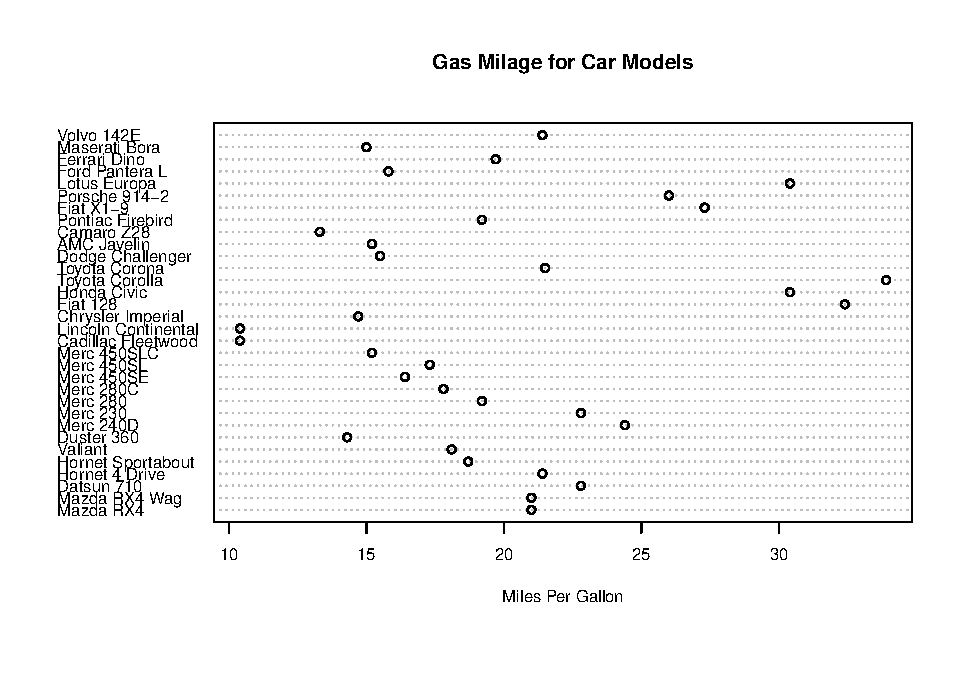
\includegraphics{l4_files/figure-pdf/unnamed-chunk-5-1.pdf}

\hypertarget{question-4}{%
\subsection{Question 4}\label{question-4}}

What does every of the below chunk options mean?

You can aplly the different options on the dot chart from the previous
question.

A. \texttt{echo=FALSE}

B. \texttt{echo=TRUE}

C. \texttt{include=FALSE}

D. \texttt{eval=FALSE,\ include=FALSE}

\hypertarget{answer-4}{%
\subsection{Answer 4}\label{answer-4}}

\begin{Shaded}
\begin{Highlighting}[]
\CommentTok{\# echo=FALSE}
\end{Highlighting}
\end{Shaded}

The echo gives us the option if to display code along with its results
or not, in this option the code will not be shown.

\begin{Shaded}
\begin{Highlighting}[]
\CommentTok{\# echo=TRUE}
\end{Highlighting}
\end{Shaded}

The echo gives us the option if to display code along with its results
or not, in this option the code will be shown.

\begin{Shaded}
\begin{Highlighting}[]
\CommentTok{\# include=FALSE}
\end{Highlighting}
\end{Shaded}

The include gives us the option if to include the chunk in the document
after running it. in this option the chunk it will not be included.

\begin{Shaded}
\begin{Highlighting}[]
\CommentTok{\# eval=FALSE, include=FALSE}
\end{Highlighting}
\end{Shaded}

The eval gives us the option if to evaluate the code and include its
results, The include gives us the option if to include the chunk in the
document after running it. In this case the the code will not be
evaluated and included in the result, and also the chunk will not be in
included in the document.

\hypertarget{question-5}{%
\subsection{Question 5}\label{question-5}}

A. Create a sentence with next parameters:

Your first name in \emph{italics} format.

Your last name in \textbf{bold}.

Your id number in \texttt{code} format.

Link to our univercity website.

\textbf{This is my example:}

\emph{Jakob} \textbf{Alderson} \texttt{123465789}
\href{https://in.bgu.ac.il/Pages/default.aspx}{BGU}

\hypertarget{question-6}{%
\subsection{Question 6}\label{question-6}}

\end{document}
